\section{Infanterietrupp / Fireteam (FT)}
\begin{wrapfigure}{R}{0.35\textwidth}
	\vspace{-50pt}
	\centering 
	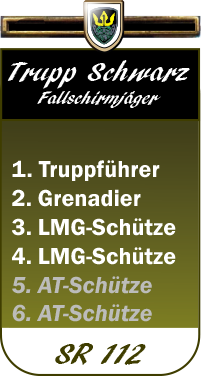
\includegraphics[width=0.2\textwidth]{../img/truppenordnung/infanterie/infanterie}
	%\caption{Beispiel eines Infantrietrupps}
	\vspace{-90pt}
\end{wrapfigure}
Die Infanterie bildet den Kernbestandteil vieler Missionen. Ein Infanterietrupp ist immer Teil eines Zuges und besteht aus 4 oder 6 Mann. Mögliche Positionen innerhalb eines Infanterietrupps sind:
\vspace{3.5cm}
\begin{longtable}{@{}P{0.4\textwidth}P{0.4\textwidth}@{}}
	\toprule
	Deutsche Bezeichnung & Englische Bezeichnung\\
	\midrule
	Truppführer (TF) & Fireteam Leader (FTL)\\
	Grenadier (GRE) & \\
	Leichter MG-Schütze (LMG) & Automatic Rifleman (AR)\\
	Mittlerer MG-Schütze & Medium Machine Gunner (MMG) \\
	MG-Assistent & Assistant Machine Gunner (AMG)\footnote{notwendig für MMG}\\ 
	Leichter Panzerabwehrschütze & Light Anti Tank (LAT)\\
	Schwerer Panzerabwehrschütze & Heavy Anti Tank (HAT)\\
	Panzerabwehr-Assistent & Assistant Anti Tank (AAT)\footnote{notwendig für HAT}\\ 
	Luftabwehrschütze & Anti-Air (AA)\\
	Pionier & Pioneer (PIO)\\
	Gefechtssanitäter & Combat Medic (CM)\\
	Schütze & Rifleman (RI)\\			
	\bottomrule					
\end{longtable}


Auf eine sinnvolle Einteilung in Buddy"=Teams (z.\,B. bei Positionen, die einen Assistenten erfordern), ist hierbei zu achten.\\
Die Kommunikation erfolgt ausschließlich über Short-Range, der Truppführer schaltet sich über seine Additional-Short-Range auf den Zugkanal auf, um sich mit der Zugführung und den anderen Truppführern im Zug abzusprechen. Die Nummer 2 im Trupp kann sich ebenfalls auf den Zugfunk aufschalten, jedoch nur mithören und nicht funken -- es sei denn, der Truppführer fällt aus und die Nummer 2 übernimmt.
